\documentclass[12pt,letterpaper]{article}
\usepackage[left=12mm,top=0.5in,bottom=5in]{geometry}
\usepackage[]{fullpage}
\usepackage[]{amsfonts}
\usepackage[]{graphicx}

\begin{document}
\date{\today}
\title{TMM Latex 12 pt}
\author{Thomas Maestas}
\maketitle
\section{Introduction} 
\begin{center}
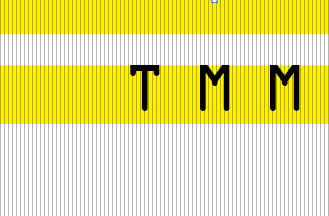
\includegraphics[scale=0.5]{../assets/TMM.jpg}
\end{center}
\begin{huge}T M M 
\end{huge}
\section{linear-functions}
\subsection{Slope-Intercept Form}
\begin{enumerate}
\item TMM is making time
\item Natural Sets denoted by $\mathbb{N}$
\item Integer Sets denoted by $\mathbb{Z}$
\item Real Number Sets denoted by $\mathbb{R}$
\end{enumerate}
\subsection{Standard Form}
\section{Motivation}
\begin{enumerate}
\item Description
\item More description
I. TMM $X1 + X4 +x5$
\end{enumerate}
\end{document}